\chapter{Appendix}\label{ch:appAlabel}

Here is the first appendix\todo{may be same as measurement}   
%\begin{tabular}{}

\begin{table}[ht]
    \begin{tabular}{|| p{0.29\linewidth} | p{0.5\linewidth}| p{0.15\linewidth}||}
        \hline
        \textbf{Term}& \textbf{Definition} & \textbf{Source} \\ [0.5ex]\hline\hline
        Software entity & Software that is to be characterized by measuring its attributes.         & FEETINGS\cite{GarciaFEETINGS}        \\ \hline
        Software entity class & The collection of all the entities that satisfy the determined objective. & FEETINGS\cite{GarciaFEETINGS}        \\ \hline
        Test Case & A representation of functionality of the software entity to be measured.  & FEETINGS\cite{GarciaFEETINGS}         \\ \hline
        Test Case Measurement & A set of energy consumption measurements of all the runs in a test case.  & FEETINGS\cite{GarciaFEETINGS}         \\ \hline
        Measurement & A set of energy consumption samples from a single test case run.       & FEETINGS\cite{GarciaFEETINGS}         \\ \hline
        Samples & Each energy consumption record taken by a measuring instrument.           & FEETINGS\cite{GarciaFEETINGS}         \\ \hline
        Device Under Test (DUT) & A device where the software entity to be measured is run.                 & FEETINGS\cite{GarciaFEETINGS}         \\ \hline
        Measuring Instrument & A method used to make energy consumption measurements.                    & FEETINGS\cite{GarciaFEETINGS}         \\ \hline
        Setup & A defined step of procedures executes at DUT startup.                     & R3\cite{Bokhari2020r3}              \\ \hline
        Batch\ & A set of test cases executed in sequence with a cool of periods.            & NEW             \\ \hline
        Configuration\ & A combinations of a DUT, measuring instrument and test case, temperature and battery.            & NEW             \\ \hline
    
    \end{tabular}
    \caption{Terminology used throughout our work.}
    \label{tab:TerminologyAlert}
    \end{table}

% \begin{figure}
%     \centering
%     \begin{tikzpicture}[]
%         \begin{axis}[ymax=1.6,
%         % axis x line=middle,
%         % axis y line=middle,
%         xlabel={x label},
%         ylabel={y label},
%         ]
%         \addplot[color=blue, mark=square,] coordinates { %% AVG value
%         (0, 1)(0.2, 1)(0.4, 0.8)(0.6, 0.5)(0.8, 0.6)(1, 0.6)
%         };
%         \addplot[color=blue, mark=square,name path=A] coordinates { %% MAX value
%         (0, 1.5)(0.2, 1.1)(0.4, 1.2)(0.6, 1.2)(0.8, 1.3)(1, 1.1)
%         };
%         \addplot[color=blue, mark=square,name path=B] coordinates { %% MIN value
%         (0, 0.9)(0.2, 0.8)(0.4, 0.5)(0.6, 0.4)(0.8, 0.2)(1,0.1)
%         };
%         \addplot [pattern=north east lines,pattern color=red] 
%         fill between [
%             of=A and B,soft clip={domain=-1.5:1.5},
%         ];
%         \end{axis}
% \end{tikzpicture}
% \caption{Graph showing average energy consumption during a run of the experiments} \label{fig:LABEL}
% \end{figure}

% \begin{figure}
%     \centering
%     \begin{tikzpicture}
%         \begin{axis}[
%             xlabel={x label},
%             ylabel={y label},
%         ]
%             \addplot [mark=none, thick, red]  coordinates {
%             (-1.5, 1)(-1, 1)(0, 1)(1, 1)(1.5, 1)
%             };
%             \addlegendentry{eh}
%             \addplot [mark=none, thick, blue] coordinates {
%             (-1.5, 2)(-1, 3)(0, 4)(1, 1)(1.5, -1)
%             };
%             \addlegendentry{oi}
%         \end{axis}
%     \end{tikzpicture} 
% \caption{Graph showing average energy consumption during a run of the experiments} \label{fig:LABEL}
% \end{figure}

% \begin{figure}
%     \centering
%     \begin{tikzpicture}[]
%         \begin{axis}[xlabel={Score}, title={Average performance comparision}, ytick={1,2,3,4},
%         yticklabels={
%             Attentive students,
%             Inattentive students, 
%             Normal students, 
%             Highly participating students
%             },
%             ]
%         \addplot+ [boxplot prepared={
%             lower whisker=25, %%  lower whisker
%             lower quartile=37, %% 25th percentile
%             median=65,  %% a median for the distribution
%             upper quartile=72, %% 75th percentile
%             upper whisker=81}, %%  upper whisker
%             ] table[row sep=\\,y index=0] {1\\ 92\\ 95\\};
%         \addplot+ [boxplot prepared={
%             lower whisker=12, 
%             lower quartile=17, 
%             median=25,
%             upper quartile=52, 
%             upper whisker=61
%             },] table[row sep=\\,y index=0] {\\};
%         \addplot+ [boxplot prepared={
%             lower whisker=12, 
%             lower quartile=25, 
%             median=50,
%             upper quartile=75, 
%             upper whisker=87},] table[row sep=\\,y index=0] {\\};
%         \addplot+ [boxplot prepared={
%             lower whisker=62, 
%             lower quartile=64, 
%             median=70,
%             upper quartile=72, 
%             upper whisker=81
%             },] table[row sep=\\,y index=0] {\\};
%         \end{axis}
%     \end{tikzpicture}
% \caption{Graph comparing performance of different duts and test cases} \label{fig:LABEL01}
% \end{figure}

% \begin{figure}
%     \centering
%     \begin{tikzpicture}[]
%         \begin{axis}[xlabel={XLABEL}, title={TITLE}, ytick={1,2,3,4},
%         yticklabels={
%             Attentive students,
%             },
%             ]
%         \addplot+ [boxplot prepared={
%             lower whisker=25, %%  lower whisker
%             lower quartile=37, %% 25th percentile
%             median=65,  %% a median for the distribution
%             upper quartile=72, %% 75th percentile
%             upper whisker=81}, %%  upper whisker
%             ] table[row sep=\\,y index=0] {1\\ 92\\ 95\\};
%         \end{axis}
%     \end{tikzpicture}
% \caption{CAPTION} \label{fig:LABEL}
% \end{figure}



% \begin{figure}
%     \centering
%     \begin{tikzpicture}[]
%         \begin{axis}[xlabel={xlabel}, title={title}, ytick={1},
%         yticklabels={
%             ytick label
%             },
%             ]
%         \addplot+ [boxplot prepared={
%                 lower whisker=25, %%  lower whisker
%                 lower quartile=37, %% 25th percentile
%                 median=65,  %% a median for the distribution
%                 upper quartile=72, %% 75th percentile
%                 upper whisker=81}, %%  upper whisker
%         ] table[row sep=\\,y index=0] {\\};
%         \end{axis}
%     \end{tikzpicture}
% \caption{caption} \label{fig:label}
% \end{figure}

% 
\begin{figure}
    \centering
    \begin{tikzpicture}
        \begin{axis}[%
        scatter/classes={%
            a={mark=o,draw=black},
            b={mark=o,draw=red}}]
        \addplot[scatter,only marks,%
            scatter src=explicit symbolic]%
        table[meta=label] {
        x y label
        0 2.8949479214654294e-05 a
        1 3.179477203046875e-05 a
        2 3.267322064601172e-05 a
        3 3.280798350852557e-05 a
        4 3.280798350852557e-05 a
        5 4.203733493201637e-05 a
        6 4.2699125166050646e-05 a
        7 4.294905342573423e-05 a
        8 4.676111584622105e-05 a
        9 4.843067177105661e-05 a
        10 4.8774191374681006e-05 a
        11 4.9445616498532656e-05 a
        12 4.9445616498532656e-05 a
        13 4.9958989436862796e-05 a
        14 5.0408826155301995e-05 a
        15 5.0408826155301995e-05 a
        16 5.193014842759746e-05 a
        17 5.634406741910958e-05 a
        18 5.6633789754044637e-05 a
        19 5.6633789754044637e-05 a
        20 5.7410217372431694e-05 a
        21 5.7410217372431694e-05 a
        22 5.921367982846027e-05 a
        23 5.921367982846027e-05 a
        24 6.0456090984576906e-05 a
        25 6.145988034834584e-05 a
        26 6.272460722809678e-05 a
        27 6.284972805645797e-05 a
        28 6.300710443137074e-05 a
        29 6.355470081318446e-05 a
        30 6.359467248323007e-05 a
        31 6.694121683315767e-05 a
        32 6.718318238640716e-05 a
        33 7.127585237345829e-05 a
        34 7.127585237345829e-05 a
        35 7.155322529164951e-05 a
        36 7.38556711976285e-05 a
        37 7.41805540625215e-05 a
        38 7.41805540625215e-05 a
        39 7.765820244366868e-05 a
        40 7.784120665026037e-05 a
        41 7.850775711089268e-05 a
        42 7.993973309373286e-05 a
        43 8.191994222015357e-05 a
        44 8.230819546665794e-05 a
        45 8.420232050680483e-05 a
        46 8.426994000106784e-05 a
        47 8.427717433224613e-05 a
        48 8.479177316626968e-05 a
        49 8.527074308148876e-05 a
        50 8.721724394873936e-05 a
        51 8.722066451929488e-05 a
        52 8.804553811338067e-05 a
        53 8.830233135155855e-05 a
        54 8.975832698738875e-05 a
        55 8.975832698738875e-05 a
        56 8.994826250782899e-05 a
        57 9.030466847320144e-05 a
        58 9.129116493983801e-05 a
        59 9.134194523707361e-05 a
        60 9.161579912448281e-05 a
        61 9.193227245685756e-05 a
        62 9.370516727749144e-05 a
        63 9.370516727749144e-05 a
        64 9.447030026752446e-05 a
        65 9.695684147183935e-05 a
        66 9.84919485426008e-05 a
        67 9.84919485426008e-05 a
        68 9.967369188253414e-05 a
        69 0.00010069773319988507 a
        70 0.00010069773319988507 a
        71 0.00010084232469055083 a
        72 0.00010512257877014406 a
        73 0.00010531121163963648 a
        74 0.00010531121163963648 a
        75 0.00010546120599483379 a
        76 0.00010572136596011746 a
        77 0.00010583143723479704 a
        78 0.00010588947949861364 a
        79 0.00010619424500734341 a
        80 0.00010702116161766447 a
        81 0.00010720818806042881 a
        82 0.00010954500810094572 a
        83 0.00010954500810094572 a
        84 0.00011073430522929063 a
        85 0.00011246416770882411 a
        86 0.0001130661635295037 a
        87 0.00011438558850046904 a
        88 0.00011469125335755415 a
        89 0.00012147392693952117 a
        90 0.00012237591171992 a
        91 0.0001224201334093466 a
        92 0.00012276203358687853 a
        93 0.0001248071419298498 a
        94 0.00012783937274188738 a
        95 0.00012853116577443856 a
        96 0.00013370751331335452 a
        97 0.00013450189840040735 a
        98 0.00013450189840040735 a
        99 0.00013535715902440975 a
        100 0.00013868052735234137 a
        101 0.00013946592819106236 a
        102 0.00013970777345427544 a
        103 0.000146505571066363 a
        104 0.00015101069658064682 a
        105 0.00015706270827900125 a
        106 0.00016013706955956582 a
        107 0.0001662494310569234 a
        108 0.0001669486955830121 a
        109 0.00017282103511564564 a
        110 0.0001741512152900111 a
        111 0.0001867419363296455 a
        112 0.00019374828758415263 a
        113 0.00019483919084249817 a
        114 0.00019699221542950795 a
        115 0.00019850109877225447 a
        116 0.00019912614342020588 a
        117 0.0002031933960156964 a
        118 0.0002232952178907816 a
        119 0.00022506654839991077 a
        120 0.000280816704139863 a
        121 0.0002832259109375601 a
        122 0.00028521681835927984 a
        123 0.00029354421334281766 a
        124 0.0003426297800563272 a
        125 0.00034744633170887413 a
        126 0.0005864789735718681 a
        127 0.0010507104872560743 a
        128 0.012726185306264882 a
        129 0.015124607637026024 a
            };
        \end{axis}
    \end{tikzpicture}
\caption{4-dist sorted graph for } \label{fig:4_dist_sorted_graph}
\end{figure}

\section*{R3 Validation for the Three DUT's}\label{app:r3_validation}

                        \begin{figure}[H]
                            \centering
                            \begin{tikzpicture}[]
                                \pgfplotsset{%
                                    width=.6\textwidth,
                                    height=0.4\textheight
                                }
                                \begin{axis}[xlabel={Average dynamic energy (Watts)}, title={workstation - IntelPowerGadget}, ytick={},
                                yticklabels={
                                    
                                    },
                                    xmin=0,xmax=80,
                                    ]
                                
                                \end{axis}
                            \end{tikzpicture}
                        \caption{R3 validation for dynamic energy measurements by IntelPowerGadget for the Cores for all DUT's on Unix and test cases where the impact of the first profiler can be seen (with outliers)} \label{fig:Fasta_Cores_R3_dynamic_energy_with_outliers_Unix_avg_watts}
                        \end{figure}
                        


                        \begin{figure}
                            \centering
                            \begin{tikzpicture}[]
                                \pgfplotsset{%
                                    width=.6\textwidth,
                                    height=0.4\textheight
                                }
                                \begin{axis}[xlabel={Average energy (Watts)}, title={workstation - HardwareMonitor}, ytick={1, 2, 3, 4, 5, 6, 7, 8, 9},
                                yticklabels={
                                    BinaryTrees - IPG, BinaryTrees - LHM, FannkuchRedux - IPG, FannkuchRedux - LHM, Nbody - IPG, Nbody - LHM, Fasta - IPG, Fasta - LHM, Fasta - CLAMP
                                    },
                                    xmin=0,xmax=80,
                                    ]
                                
                                    \addplot+ [boxplot prepared={
                                    lower whisker=49.00751457176233,
                                    lower quartile=49.61370310263379,
                                    median=49.86635993972493,
                                    upper quartile=50.05370322590609,
                                    upper whisker=50.30167874146812},
                                    ] table[row sep=\\,y index=0] {\\};
                                    
                                    \addplot+ [boxplot prepared={
                                    lower whisker=49.96582370797222,
                                    lower quartile=50.10332634853504,
                                    median=50.19369566319231,
                                    upper quartile=50.50935073182443,
                                    upper whisker=51.32271063431183},
                                    ] table[row sep=\\,y index=0] {\\};
                                    
                                    \addplot+ [boxplot prepared={
                                    lower whisker=39.19880796803349,
                                    lower quartile=40.104491133132555,
                                    median=40.8449788838508,
                                    upper quartile=41.00115047177299,
                                    upper whisker=41.88854450579453},
                                    ] table[row sep=\\,y index=0] {\\};
                                    
                                    \addplot+ [boxplot prepared={
                                    lower whisker=39.568400712129986,
                                    lower quartile=40.27079510593521,
                                    median=40.512046206147346,
                                    upper quartile=41.48040545003127,
                                    upper whisker=42.16788282269731},
                                    ] table[row sep=\\,y index=0] {\\};
                                    
                                    \addplot+ [boxplot prepared={
                                    lower whisker=17.39534220186832,
                                    lower quartile=17.552153462160753,
                                    median=17.818640525522827,
                                    upper quartile=18.222217711877704,
                                    upper whisker=18.67722321161588},
                                    ] table[row sep=\\,y index=0] {\\};
                                    
                                    \addplot+ [boxplot prepared={
                                    lower whisker=17.850501152784698,
                                    lower quartile=18.106524757871732,
                                    median=18.312372182960253,
                                    upper quartile=18.45014417620998,
                                    upper whisker=18.501941485780637},
                                    ] table[row sep=\\,y index=0] {\\};
                                    
                                    \addplot+ [boxplot prepared={
                                    lower whisker=28.346426039236473,
                                    lower quartile=28.353171180147218,
                                    median=28.484940519278002,
                                    upper quartile=28.526442555499866,
                                    upper whisker=28.89112647916421},
                                    ] table[row sep=\\,y index=0] {\\};
                                    
                                    \addplot+ [boxplot prepared={
                                    lower whisker=27.861227463369577,
                                    lower quartile=28.338770068312684,
                                    median=28.531829140241964,
                                    upper quartile=28.912113200985477,
                                    upper whisker=31.36141039021059},
                                    ] table[row sep=\\,y index=0] {\\};
                                    
                                    \addplot+ [boxplot prepared={
                                    lower whisker=28.538517798231357,
                                    lower quartile=28.59400314276051,
                                    median=28.63167393595622,
                                    upper quartile=28.640270552740223,
                                    upper whisker=28.693943892556323},
                                    ] table[row sep=\\,y index=0] {\\};
                                    
                                \end{axis}
                            \end{tikzpicture}
                        \caption{R3 validation for energy measurements by HardwareMonitor for the Cores for all DUT's on Win32NT and test cases where the impact of the first profiler can be seen (with outliers)} \label{fig:PowerKomplett_HardwareMonitor_Cores_R3_energy_with_outliers_Win32NT_avg_watts_exp2}
                        \end{figure}
                        

                        \begin{figure}[H]
                            \centering
                            \begin{tikzpicture}[]
                                \pgfplotsset{%
                                    width=.6\textwidth,
                                    height=0.4\textheight
                                }
                                \begin{axis}[xlabel={Average dynamic energy (Watts)}, title={workstation - IntelPowerGadget}, ytick={},
                                yticklabels={
                                    
                                    },
                                    xmin=0,xmax=80,
                                    ]
                                
                                \end{axis}
                            \end{tikzpicture}
                        \caption{R3 validation for dynamic energy measurements by IntelPowerGadget for the Cores for all DUT's on Unix and test cases where the impact of the first profiler can be seen (with outliers)} \label{fig:Fasta_Cores_R3_dynamic_energy_with_outliers_Unix_avg_watts}
                        \end{figure}
                        


                        \begin{figure}
                            \centering
                            \begin{tikzpicture}[]
                                \pgfplotsset{%
                                    width=.6\textwidth,
                                    height=0.4\textheight
                                }
                                \begin{axis}[xlabel={Average energy (Watts)}, title={workstation - HardwareMonitor}, ytick={1, 2, 3, 4, 5, 6, 7, 8, 9},
                                yticklabels={
                                    BinaryTrees - IPG, BinaryTrees - LHM, FannkuchRedux - IPG, FannkuchRedux - LHM, Nbody - IPG, Nbody - LHM, Fasta - IPG, Fasta - LHM, Fasta - CLAMP
                                    },
                                    xmin=0,xmax=80,
                                    ]
                                
                                    \addplot+ [boxplot prepared={
                                    lower whisker=49.00751457176233,
                                    lower quartile=49.61370310263379,
                                    median=49.86635993972493,
                                    upper quartile=50.05370322590609,
                                    upper whisker=50.30167874146812},
                                    ] table[row sep=\\,y index=0] {\\};
                                    
                                    \addplot+ [boxplot prepared={
                                    lower whisker=49.96582370797222,
                                    lower quartile=50.10332634853504,
                                    median=50.19369566319231,
                                    upper quartile=50.50935073182443,
                                    upper whisker=51.32271063431183},
                                    ] table[row sep=\\,y index=0] {\\};
                                    
                                    \addplot+ [boxplot prepared={
                                    lower whisker=39.19880796803349,
                                    lower quartile=40.104491133132555,
                                    median=40.8449788838508,
                                    upper quartile=41.00115047177299,
                                    upper whisker=41.88854450579453},
                                    ] table[row sep=\\,y index=0] {\\};
                                    
                                    \addplot+ [boxplot prepared={
                                    lower whisker=39.568400712129986,
                                    lower quartile=40.27079510593521,
                                    median=40.512046206147346,
                                    upper quartile=41.48040545003127,
                                    upper whisker=42.16788282269731},
                                    ] table[row sep=\\,y index=0] {\\};
                                    
                                    \addplot+ [boxplot prepared={
                                    lower whisker=17.39534220186832,
                                    lower quartile=17.552153462160753,
                                    median=17.818640525522827,
                                    upper quartile=18.222217711877704,
                                    upper whisker=18.67722321161588},
                                    ] table[row sep=\\,y index=0] {\\};
                                    
                                    \addplot+ [boxplot prepared={
                                    lower whisker=17.850501152784698,
                                    lower quartile=18.106524757871732,
                                    median=18.312372182960253,
                                    upper quartile=18.45014417620998,
                                    upper whisker=18.501941485780637},
                                    ] table[row sep=\\,y index=0] {\\};
                                    
                                    \addplot+ [boxplot prepared={
                                    lower whisker=28.346426039236473,
                                    lower quartile=28.353171180147218,
                                    median=28.484940519278002,
                                    upper quartile=28.526442555499866,
                                    upper whisker=28.89112647916421},
                                    ] table[row sep=\\,y index=0] {\\};
                                    
                                    \addplot+ [boxplot prepared={
                                    lower whisker=27.861227463369577,
                                    lower quartile=28.338770068312684,
                                    median=28.531829140241964,
                                    upper quartile=28.912113200985477,
                                    upper whisker=31.36141039021059},
                                    ] table[row sep=\\,y index=0] {\\};
                                    
                                    \addplot+ [boxplot prepared={
                                    lower whisker=28.538517798231357,
                                    lower quartile=28.59400314276051,
                                    median=28.63167393595622,
                                    upper quartile=28.640270552740223,
                                    upper whisker=28.693943892556323},
                                    ] table[row sep=\\,y index=0] {\\};
                                    
                                \end{axis}
                            \end{tikzpicture}
                        \caption{R3 validation for energy measurements by HardwareMonitor for the Cores for all DUT's on Win32NT and test cases where the impact of the first profiler can be seen (with outliers)} \label{fig:PowerKomplett_HardwareMonitor_Cores_R3_energy_with_outliers_Win32NT_avg_watts_exp2}
                        \end{figure}
                        

                        \begin{figure}[H]
                            \centering
                            \begin{tikzpicture}[]
                                \pgfplotsset{%
                                    width=.6\textwidth,
                                    height=0.4\textheight
                                }
                                \begin{axis}[xlabel={Average dynamic energy (Watts)}, title={workstation - IntelPowerGadget}, ytick={},
                                yticklabels={
                                    
                                    },
                                    xmin=0,xmax=80,
                                    ]
                                
                                \end{axis}
                            \end{tikzpicture}
                        \caption{R3 validation for dynamic energy measurements by IntelPowerGadget for the Cores for all DUT's on Unix and test cases where the impact of the first profiler can be seen (with outliers)} \label{fig:Fasta_Cores_R3_dynamic_energy_with_outliers_Unix_avg_watts}
                        \end{figure}
                        


\section{The Battery Levels Impact on Performance}\label{app:charge}

                            \begin{figure}
                                \centering
                                \begin{tikzpicture}[]
                                    \pgfplotsset{%
                                        width=.85\textwidth,
                                        height=.15\textheight
                                    }
                                    \begin{axis}[xlabel={Average energy consumption (Watts)}, title={Cores - BinaryTrees - Energy - without outliers}, ytick={},
                                    yticklabels={
                                        
                                        },
                                        xmin=0,xmax=20,
                                        ]
                                    
                                    \end{axis}
                                \end{tikzpicture}
                            \caption{A comparison of of Cores energy consumption for test case BinaryTrees for the Surface4Pro,  experiment \#2 (without outliers)} \label{fig:BinaryTrees_Cores_comparison_energy_without_outliers_Surface4Pro_avg_watts_exp2}
                            \end{figure}
                            

                            \begin{figure}
                                \centering
                                \begin{tikzpicture}[]
                                    \pgfplotsset{%
                                        width=.7\textwidth,
                                        height=.2\textheight
                                    }
                                    \begin{axis}[xlabel={Average energy consumption (Watts)}, title={Cores - Fasta - Energy - without outliers}, ytick={1, 2},
                                    yticklabels={
                                        IntelPowerGadget , HardwareMonitor 
                                        },
                                        xmin=0,xmax=80,
                                        ]
                                    
                                    \addplot+ [boxplot prepared={
                                    lower whisker=54.22445449466433,
                                    lower quartile=54.45751347572185,
                                    median=54.54624547297937,
                                    upper quartile=54.72020125409266,
                                    upper whisker=55.103791721157386},
                                    ] table[row sep=\\,y index=0] {\\};
                                    
                                    \addplot+ [boxplot prepared={
                                    lower whisker=51.45082608392138,
                                    lower quartile=51.933860038023106,
                                    median=52.121433545941585,
                                    upper quartile=52.479201309170854,
                                    upper whisker=54.95103920614709},
                                    ] table[row sep=\\,y index=0] {\\};
                                    
                                    \end{axis}
                                \end{tikzpicture}
                            \caption{A comparison of of Cores energy consumption for test case Fasta for the workstation (without outliers)} \label{fig:Fasta_Cores_comparison_energy_without_outliers_PowerKomplett_avg_watts_exp2}
                            \end{figure}
                            

                \begin{figure}[H]
                    \centering
                    \begin{tikzpicture}
                        \pgfplotsset{%
                            width=1\textwidth,
                            height=0.4\textheight
                        }
                        \begin{axis}[
                            xlabel={Start battery level},
                            ylabel={Average dynamic energy (watt)},
                            ymin=0,ymax=20,
                        ]
                        
                            \addplot [mark=none, ultra thick, red]  coordinates {
                            (40, 0.006595684402444291)(45, 0.007295220674193181)(50, 0.007999659608910881)(55, 0.007202467971243639)(60, 0.007280865079495958)(65, 0.006858423509955077)(70, 0.008369444141141925)(75, 0.007144940647010992)(80, 0.004753236834232667)
                            };
                            \addlegendentry{Surface4Pro - IntelPowerGadget}
                            
                            \addplot [mark=none, ultra thick, blue]  coordinates {
                            (40, 0.002385328427460912)(45, 0.0017856511573015649)(50, 0.0025901992189954056)(55, 0.00210998144366709)(60, 0.00286452646862575)(65, 0.0020038487280194628)(70, 0.002908483770774353)(75, 0.0005098111150931342)(80, -0.005995916826693459)
                            };
                            \addlegendentry{Surface4Pro - HardwareMonitor}
                            
                            \addplot [mark=none, ultra thick, orange]  coordinates {
                            (50, 251.8661014299577)(55, 214.7597259251014)(60, 162.23880995564176)(65, 107.43421593849766)(70, 53.9187387386668)(75, 0.7554852536149699)(80, -44.463085003568885)
                            };
                            \addlegendentry{Surface4Pro - RAPL}
                            
                            \addplot [mark=none, dashdotted, red]  coordinates {
                            (40, -0.004038062354887025)(45, -0.004312668500277529)(50, -0.003808663911021498)(55, -0.0037057407527755254)(60, -0.004478257932982471)(65, -0.0026308734995501644)(70, -0.0034090674446925874)(75, -0.003041497079697436)(80, -0.0020334307266356875)
                            };
                            \addlegendentry{SurfaceBook - IntelPowerGadget}
                            
                            \addplot [mark=none, dashdotted, blue]  coordinates {
                            (40, -0.002443518930616523)(45, -0.0029256880137447055)(50, -0.002551777773312929)(55, -0.0027567211782433486)(60, -0.002206859154402231)(65, -0.0026388300848279207)(70, -0.0024597736945479324)(75, -0.002445350799195827)(80, -0.000541271265011134)
                            };
                            \addlegendentry{SurfaceBook - HardwareMonitor}
                            
                            \addplot [mark=none, dashdotted, orange]  coordinates {
                            (40, 101.92702155010147)(45, 86.7212700795567)(50, 69.40754598562454)(55, 51.343785407669614)(60, 32.443112755251185)(65, 14.52577919077786)(70, -4.520517378551423)(75, -23.811706977384954)(80, -35.700372165212755)
                            };
                            \addlegendentry{SurfaceBook - RAPL}
                            
                        \end{axis}
                    \end{tikzpicture} 
                \caption{A graph illustrating the energy consumption of Dram for test case Nbody with regards to the battey level of the DUT (with outliers)} \label{fig:Nbody_Dram_charge}
                \end{figure}
                

\section{The Temperatures Levels Impact on Performance}\label{app:temperature}

                            \begin{figure}
                                \centering
                                \begin{tikzpicture}[]
                                    \pgfplotsset{%
                                        width=.85\textwidth,
                                        height=.15\textheight
                                    }
                                    \begin{axis}[xlabel={Average energy consumption (Watts)}, title={Cores - BinaryTrees - Energy - without outliers}, ytick={},
                                    yticklabels={
                                        
                                        },
                                        xmin=0,xmax=20,
                                        ]
                                    
                                    \end{axis}
                                \end{tikzpicture}
                            \caption{A comparison of of Cores energy consumption for test case BinaryTrees for the Surface4Pro,  experiment \#2 (without outliers)} \label{fig:BinaryTrees_Cores_comparison_energy_without_outliers_Surface4Pro_avg_watts_exp2}
                            \end{figure}
                            

                            \begin{figure}
                                \centering
                                \begin{tikzpicture}[]
                                    \pgfplotsset{%
                                        width=.7\textwidth,
                                        height=.2\textheight
                                    }
                                    \begin{axis}[xlabel={Average energy consumption (Watts)}, title={Cores - Fasta - Energy - without outliers}, ytick={1, 2},
                                    yticklabels={
                                        IntelPowerGadget , HardwareMonitor 
                                        },
                                        xmin=0,xmax=80,
                                        ]
                                    
                                    \addplot+ [boxplot prepared={
                                    lower whisker=54.22445449466433,
                                    lower quartile=54.45751347572185,
                                    median=54.54624547297937,
                                    upper quartile=54.72020125409266,
                                    upper whisker=55.103791721157386},
                                    ] table[row sep=\\,y index=0] {\\};
                                    
                                    \addplot+ [boxplot prepared={
                                    lower whisker=51.45082608392138,
                                    lower quartile=51.933860038023106,
                                    median=52.121433545941585,
                                    upper quartile=52.479201309170854,
                                    upper whisker=54.95103920614709},
                                    ] table[row sep=\\,y index=0] {\\};
                                    
                                    \end{axis}
                                \end{tikzpicture}
                            \caption{A comparison of of Cores energy consumption for test case Fasta for the workstation (without outliers)} \label{fig:Fasta_Cores_comparison_energy_without_outliers_PowerKomplett_avg_watts_exp2}
                            \end{figure}
                            

                \begin{figure}[H]
                    \centering
                    \begin{tikzpicture}
                        \pgfplotsset{%
                            width=1\textwidth,
                            height=0.4\textheight
                        }
                        \begin{axis}[
                            xlabel={Start battery level},
                            ylabel={Average dynamic energy (watt)},
                            ymin=0,ymax=20,
                        ]
                        
                            \addplot [mark=none, ultra thick, red]  coordinates {
                            (40, 0.006595684402444291)(45, 0.007295220674193181)(50, 0.007999659608910881)(55, 0.007202467971243639)(60, 0.007280865079495958)(65, 0.006858423509955077)(70, 0.008369444141141925)(75, 0.007144940647010992)(80, 0.004753236834232667)
                            };
                            \addlegendentry{Surface4Pro - IntelPowerGadget}
                            
                            \addplot [mark=none, ultra thick, blue]  coordinates {
                            (40, 0.002385328427460912)(45, 0.0017856511573015649)(50, 0.0025901992189954056)(55, 0.00210998144366709)(60, 0.00286452646862575)(65, 0.0020038487280194628)(70, 0.002908483770774353)(75, 0.0005098111150931342)(80, -0.005995916826693459)
                            };
                            \addlegendentry{Surface4Pro - HardwareMonitor}
                            
                            \addplot [mark=none, ultra thick, orange]  coordinates {
                            (50, 251.8661014299577)(55, 214.7597259251014)(60, 162.23880995564176)(65, 107.43421593849766)(70, 53.9187387386668)(75, 0.7554852536149699)(80, -44.463085003568885)
                            };
                            \addlegendentry{Surface4Pro - RAPL}
                            
                            \addplot [mark=none, dashdotted, red]  coordinates {
                            (40, -0.004038062354887025)(45, -0.004312668500277529)(50, -0.003808663911021498)(55, -0.0037057407527755254)(60, -0.004478257932982471)(65, -0.0026308734995501644)(70, -0.0034090674446925874)(75, -0.003041497079697436)(80, -0.0020334307266356875)
                            };
                            \addlegendentry{SurfaceBook - IntelPowerGadget}
                            
                            \addplot [mark=none, dashdotted, blue]  coordinates {
                            (40, -0.002443518930616523)(45, -0.0029256880137447055)(50, -0.002551777773312929)(55, -0.0027567211782433486)(60, -0.002206859154402231)(65, -0.0026388300848279207)(70, -0.0024597736945479324)(75, -0.002445350799195827)(80, -0.000541271265011134)
                            };
                            \addlegendentry{SurfaceBook - HardwareMonitor}
                            
                            \addplot [mark=none, dashdotted, orange]  coordinates {
                            (40, 101.92702155010147)(45, 86.7212700795567)(50, 69.40754598562454)(55, 51.343785407669614)(60, 32.443112755251185)(65, 14.52577919077786)(70, -4.520517378551423)(75, -23.811706977384954)(80, -35.700372165212755)
                            };
                            \addlegendentry{SurfaceBook - RAPL}
                            
                        \end{axis}
                    \end{tikzpicture} 
                \caption{A graph illustrating the energy consumption of Dram for test case Nbody with regards to the battey level of the DUT (with outliers)} \label{fig:Nbody_Dram_charge}
                \end{figure}
                


% 
                            \begin{figure}
                                \centering
                                \begin{tikzpicture}[]
                                    \pgfplotsset{%
                                        width=.7\textwidth,
                                        height=.2\textheight
                                    }
                                    \begin{axis}[xlabel={Average energy consumption (Watts)}, title={Cores - Fasta - Energy - without outliers}, ytick={1, 2},
                                    yticklabels={
                                        IntelPowerGadget , HardwareMonitor 
                                        },
                                        xmin=0,xmax=80,
                                        ]
                                    
                                    \addplot+ [boxplot prepared={
                                    lower whisker=54.22445449466433,
                                    lower quartile=54.45751347572185,
                                    median=54.54624547297937,
                                    upper quartile=54.72020125409266,
                                    upper whisker=55.103791721157386},
                                    ] table[row sep=\\,y index=0] {\\};
                                    
                                    \addplot+ [boxplot prepared={
                                    lower whisker=51.45082608392138,
                                    lower quartile=51.933860038023106,
                                    median=52.121433545941585,
                                    upper quartile=52.479201309170854,
                                    upper whisker=54.95103920614709},
                                    ] table[row sep=\\,y index=0] {\\};
                                    
                                    \end{axis}
                                \end{tikzpicture}
                            \caption{A comparison of of Cores energy consumption for test case Fasta for the workstation (without outliers)} \label{fig:Fasta_Cores_comparison_energy_without_outliers_PowerKomplett_avg_watts_exp2}
                            \end{figure}
                            
% 
                            \begin{figure}
                                \centering
                                \begin{tikzpicture}[]
                                    \pgfplotsset{%
                                        width=.7\textwidth,
                                        height=.2\textheight
                                    }
                                    \begin{axis}[xlabel={Average energy consumption (Watts)}, title={Cores - Fasta - Energy - without outliers}, ytick={1, 2},
                                    yticklabels={
                                        IntelPowerGadget , HardwareMonitor 
                                        },
                                        xmin=0,xmax=80,
                                        ]
                                    
                                    \addplot+ [boxplot prepared={
                                    lower whisker=54.22445449466433,
                                    lower quartile=54.45751347572185,
                                    median=54.54624547297937,
                                    upper quartile=54.72020125409266,
                                    upper whisker=55.103791721157386},
                                    ] table[row sep=\\,y index=0] {\\};
                                    
                                    \addplot+ [boxplot prepared={
                                    lower whisker=51.45082608392138,
                                    lower quartile=51.933860038023106,
                                    median=52.121433545941585,
                                    upper quartile=52.479201309170854,
                                    upper whisker=54.95103920614709},
                                    ] table[row sep=\\,y index=0] {\\};
                                    
                                    \end{axis}
                                \end{tikzpicture}
                            \caption{A comparison of of Cores energy consumption for test case Fasta for the workstation (without outliers)} \label{fig:Fasta_Cores_comparison_energy_without_outliers_PowerKomplett_avg_watts_exp2}
                            \end{figure}
                            
% 
                            \begin{figure}
                                \centering
                                \begin{tikzpicture}[]
                                    \pgfplotsset{%
                                        width=.7\textwidth,
                                        height=.2\textheight
                                    }
                                    \begin{axis}[xlabel={Average energy consumption (Watts)}, title={Cores - Fasta - Energy - without outliers}, ytick={1, 2},
                                    yticklabels={
                                        IntelPowerGadget , HardwareMonitor 
                                        },
                                        xmin=0,xmax=80,
                                        ]
                                    
                                    \addplot+ [boxplot prepared={
                                    lower whisker=54.22445449466433,
                                    lower quartile=54.45751347572185,
                                    median=54.54624547297937,
                                    upper quartile=54.72020125409266,
                                    upper whisker=55.103791721157386},
                                    ] table[row sep=\\,y index=0] {\\};
                                    
                                    \addplot+ [boxplot prepared={
                                    lower whisker=51.45082608392138,
                                    lower quartile=51.933860038023106,
                                    median=52.121433545941585,
                                    upper quartile=52.479201309170854,
                                    upper whisker=54.95103920614709},
                                    ] table[row sep=\\,y index=0] {\\};
                                    
                                    \end{axis}
                                \end{tikzpicture}
                            \caption{A comparison of of Cores energy consumption for test case Fasta for the workstation (without outliers)} \label{fig:Fasta_Cores_comparison_energy_without_outliers_PowerKomplett_avg_watts_exp2}
                            \end{figure}
                            
% 
                            \begin{figure}
                                \centering
                                \begin{tikzpicture}[]
                                    \pgfplotsset{%
                                        width=.7\textwidth,
                                        height=.2\textheight
                                    }
                                    \begin{axis}[xlabel={Average energy consumption (Watts)}, title={Cores - Fasta - Energy - without outliers}, ytick={1, 2},
                                    yticklabels={
                                        IntelPowerGadget , HardwareMonitor 
                                        },
                                        xmin=0,xmax=80,
                                        ]
                                    
                                    \addplot+ [boxplot prepared={
                                    lower whisker=54.22445449466433,
                                    lower quartile=54.45751347572185,
                                    median=54.54624547297937,
                                    upper quartile=54.72020125409266,
                                    upper whisker=55.103791721157386},
                                    ] table[row sep=\\,y index=0] {\\};
                                    
                                    \addplot+ [boxplot prepared={
                                    lower whisker=51.45082608392138,
                                    lower quartile=51.933860038023106,
                                    median=52.121433545941585,
                                    upper quartile=52.479201309170854,
                                    upper whisker=54.95103920614709},
                                    ] table[row sep=\\,y index=0] {\\};
                                    
                                    \end{axis}
                                \end{tikzpicture}
                            \caption{A comparison of of Cores energy consumption for test case Fasta for the workstation (without outliers)} \label{fig:Fasta_Cores_comparison_energy_without_outliers_PowerKomplett_avg_watts_exp2}
                            \end{figure}
                            
% 
                            \begin{figure}
                                \centering
                                \begin{tikzpicture}[]
                                    \pgfplotsset{%
                                        width=.7\textwidth,
                                        height=.2\textheight
                                    }
                                    \begin{axis}[xlabel={Average energy consumption (Watts)}, title={Cores - Fasta - Energy - without outliers}, ytick={1, 2},
                                    yticklabels={
                                        IntelPowerGadget , HardwareMonitor 
                                        },
                                        xmin=0,xmax=80,
                                        ]
                                    
                                    \addplot+ [boxplot prepared={
                                    lower whisker=54.22445449466433,
                                    lower quartile=54.45751347572185,
                                    median=54.54624547297937,
                                    upper quartile=54.72020125409266,
                                    upper whisker=55.103791721157386},
                                    ] table[row sep=\\,y index=0] {\\};
                                    
                                    \addplot+ [boxplot prepared={
                                    lower whisker=51.45082608392138,
                                    lower quartile=51.933860038023106,
                                    median=52.121433545941585,
                                    upper quartile=52.479201309170854,
                                    upper whisker=54.95103920614709},
                                    ] table[row sep=\\,y index=0] {\\};
                                    
                                    \end{axis}
                                \end{tikzpicture}
                            \caption{A comparison of of Cores energy consumption for test case Fasta for the workstation (without outliers)} \label{fig:Fasta_Cores_comparison_energy_without_outliers_PowerKomplett_avg_watts_exp2}
                            \end{figure}
                            

% 
                            \begin{figure}
                                \centering
                                \begin{tikzpicture}[]
                                    \pgfplotsset{%
                                        width=.85\textwidth,
                                        height=.15\textheight
                                    }
                                    \begin{axis}[xlabel={Average energy consumption (Watts)}, title={Cores - BinaryTrees - Energy - without outliers}, ytick={},
                                    yticklabels={
                                        
                                        },
                                        xmin=0,xmax=20,
                                        ]
                                    
                                    \end{axis}
                                \end{tikzpicture}
                            \caption{A comparison of of Cores energy consumption for test case BinaryTrees for the Surface4Pro,  experiment \#2 (without outliers)} \label{fig:BinaryTrees_Cores_comparison_energy_without_outliers_Surface4Pro_avg_watts_exp2}
                            \end{figure}
                            
% 
                            \begin{figure}
                                \centering
                                \begin{tikzpicture}[]
                                    \pgfplotsset{%
                                        width=.7\textwidth,
                                        height=.2\textheight
                                    }
                                    \begin{axis}[xlabel={Average energy consumption (Watts)}, title={Cores - Fasta - Energy - without outliers}, ytick={1, 2},
                                    yticklabels={
                                        IntelPowerGadget , HardwareMonitor 
                                        },
                                        xmin=0,xmax=80,
                                        ]
                                    
                                    \addplot+ [boxplot prepared={
                                    lower whisker=54.22445449466433,
                                    lower quartile=54.45751347572185,
                                    median=54.54624547297937,
                                    upper quartile=54.72020125409266,
                                    upper whisker=55.103791721157386},
                                    ] table[row sep=\\,y index=0] {\\};
                                    
                                    \addplot+ [boxplot prepared={
                                    lower whisker=51.45082608392138,
                                    lower quartile=51.933860038023106,
                                    median=52.121433545941585,
                                    upper quartile=52.479201309170854,
                                    upper whisker=54.95103920614709},
                                    ] table[row sep=\\,y index=0] {\\};
                                    
                                    \end{axis}
                                \end{tikzpicture}
                            \caption{A comparison of of Cores energy consumption for test case Fasta for the workstation (without outliers)} \label{fig:Fasta_Cores_comparison_energy_without_outliers_PowerKomplett_avg_watts_exp2}
                            \end{figure}
                            
% 
                \begin{figure}[H]
                    \centering
                    \begin{tikzpicture}
                        \pgfplotsset{%
                            width=1\textwidth,
                            height=0.4\textheight
                        }
                        \begin{axis}[
                            xlabel={Start battery level},
                            ylabel={Average dynamic energy (watt)},
                            ymin=0,ymax=20,
                        ]
                        
                            \addplot [mark=none, ultra thick, red]  coordinates {
                            (40, 0.006595684402444291)(45, 0.007295220674193181)(50, 0.007999659608910881)(55, 0.007202467971243639)(60, 0.007280865079495958)(65, 0.006858423509955077)(70, 0.008369444141141925)(75, 0.007144940647010992)(80, 0.004753236834232667)
                            };
                            \addlegendentry{Surface4Pro - IntelPowerGadget}
                            
                            \addplot [mark=none, ultra thick, blue]  coordinates {
                            (40, 0.002385328427460912)(45, 0.0017856511573015649)(50, 0.0025901992189954056)(55, 0.00210998144366709)(60, 0.00286452646862575)(65, 0.0020038487280194628)(70, 0.002908483770774353)(75, 0.0005098111150931342)(80, -0.005995916826693459)
                            };
                            \addlegendentry{Surface4Pro - HardwareMonitor}
                            
                            \addplot [mark=none, ultra thick, orange]  coordinates {
                            (50, 251.8661014299577)(55, 214.7597259251014)(60, 162.23880995564176)(65, 107.43421593849766)(70, 53.9187387386668)(75, 0.7554852536149699)(80, -44.463085003568885)
                            };
                            \addlegendentry{Surface4Pro - RAPL}
                            
                            \addplot [mark=none, dashdotted, red]  coordinates {
                            (40, -0.004038062354887025)(45, -0.004312668500277529)(50, -0.003808663911021498)(55, -0.0037057407527755254)(60, -0.004478257932982471)(65, -0.0026308734995501644)(70, -0.0034090674446925874)(75, -0.003041497079697436)(80, -0.0020334307266356875)
                            };
                            \addlegendentry{SurfaceBook - IntelPowerGadget}
                            
                            \addplot [mark=none, dashdotted, blue]  coordinates {
                            (40, -0.002443518930616523)(45, -0.0029256880137447055)(50, -0.002551777773312929)(55, -0.0027567211782433486)(60, -0.002206859154402231)(65, -0.0026388300848279207)(70, -0.0024597736945479324)(75, -0.002445350799195827)(80, -0.000541271265011134)
                            };
                            \addlegendentry{SurfaceBook - HardwareMonitor}
                            
                            \addplot [mark=none, dashdotted, orange]  coordinates {
                            (40, 101.92702155010147)(45, 86.7212700795567)(50, 69.40754598562454)(55, 51.343785407669614)(60, 32.443112755251185)(65, 14.52577919077786)(70, -4.520517378551423)(75, -23.811706977384954)(80, -35.700372165212755)
                            };
                            \addlegendentry{SurfaceBook - RAPL}
                            
                        \end{axis}
                    \end{tikzpicture} 
                \caption{A graph illustrating the energy consumption of Dram for test case Nbody with regards to the battey level of the DUT (with outliers)} \label{fig:Nbody_Dram_charge}
                \end{figure}
                
% 
                            \begin{figure}
                                \centering
                                \begin{tikzpicture}[]
                                    \pgfplotsset{%
                                        width=.85\textwidth,
                                        height=.15\textheight
                                    }
                                    \begin{axis}[xlabel={Average energy consumption (Watts)}, title={Cores - FannkuchRedux - Energy - without outliers}, ytick={},
                                    yticklabels={
                                        
                                        },
                                        xmin=0,xmax=20,
                                        ]
                                    
                                    \end{axis}
                                \end{tikzpicture}
                            \caption{A comparison of of Cores energy consumption for test case FannkuchRedux for the Surface4Pro,  experiment \#2 (without outliers)} \label{fig:FannkuchRedux_Cores_comparison_energy_without_outliers_Surface4Pro_avg_watts_exp2}
                            \end{figure}
                            

% 
                            \begin{figure}
                                \centering
                                \begin{tikzpicture}[]
                                    \pgfplotsset{%
                                        width=.85\textwidth,
                                        height=.15\textheight
                                    }
                                    \begin{axis}[xlabel={Average energy consumption (Watts)}, title={Cores - FannkuchRedux - Energy - without outliers}, ytick={},
                                    yticklabels={
                                        
                                        },
                                        xmin=0,xmax=20,
                                        ]
                                    
                                    \end{axis}
                                \end{tikzpicture}
                            \caption{A comparison of of Cores energy consumption for test case FannkuchRedux for the Surface4Pro,  experiment \#2 (without outliers)} \label{fig:FannkuchRedux_Cores_comparison_energy_without_outliers_Surface4Pro_avg_watts_exp2}
                            \end{figure}
                            
% 
                            \begin{figure}
                                \centering
                                \begin{tikzpicture}[]
                                    \pgfplotsset{%
                                        width=.85\textwidth,
                                        height=.15\textheight
                                    }
                                    \begin{axis}[xlabel={Average energy consumption (Watts)}, title={Cores - BinaryTrees - Energy - without outliers}, ytick={},
                                    yticklabels={
                                        
                                        },
                                        xmin=0,xmax=20,
                                        ]
                                    
                                    \end{axis}
                                \end{tikzpicture}
                            \caption{A comparison of of Cores energy consumption for test case BinaryTrees for the Surface4Pro,  experiment \#2 (without outliers)} \label{fig:BinaryTrees_Cores_comparison_energy_without_outliers_Surface4Pro_avg_watts_exp2}
                            \end{figure}
                            
% 
                            \begin{figure}
                                \centering
                                \begin{tikzpicture}[]
                                    \pgfplotsset{%
                                        width=.7\textwidth,
                                        height=.2\textheight
                                    }
                                    \begin{axis}[xlabel={Average energy consumption (Watts)}, title={Cores - Fasta - Energy - without outliers}, ytick={1, 2},
                                    yticklabels={
                                        IntelPowerGadget , HardwareMonitor 
                                        },
                                        xmin=0,xmax=80,
                                        ]
                                    
                                    \addplot+ [boxplot prepared={
                                    lower whisker=54.22445449466433,
                                    lower quartile=54.45751347572185,
                                    median=54.54624547297937,
                                    upper quartile=54.72020125409266,
                                    upper whisker=55.103791721157386},
                                    ] table[row sep=\\,y index=0] {\\};
                                    
                                    \addplot+ [boxplot prepared={
                                    lower whisker=51.45082608392138,
                                    lower quartile=51.933860038023106,
                                    median=52.121433545941585,
                                    upper quartile=52.479201309170854,
                                    upper whisker=54.95103920614709},
                                    ] table[row sep=\\,y index=0] {\\};
                                    
                                    \end{axis}
                                \end{tikzpicture}
                            \caption{A comparison of of Cores energy consumption for test case Fasta for the workstation (without outliers)} \label{fig:Fasta_Cores_comparison_energy_without_outliers_PowerKomplett_avg_watts_exp2}
                            \end{figure}
                            
% 
                \begin{figure}[H]
                    \centering
                    \begin{tikzpicture}
                        \pgfplotsset{%
                            width=1\textwidth,
                            height=0.4\textheight
                        }
                        \begin{axis}[
                            xlabel={Start battery level},
                            ylabel={Average dynamic energy (watt)},
                            ymin=0,ymax=20,
                        ]
                        
                            \addplot [mark=none, ultra thick, red]  coordinates {
                            (40, 0.006595684402444291)(45, 0.007295220674193181)(50, 0.007999659608910881)(55, 0.007202467971243639)(60, 0.007280865079495958)(65, 0.006858423509955077)(70, 0.008369444141141925)(75, 0.007144940647010992)(80, 0.004753236834232667)
                            };
                            \addlegendentry{Surface4Pro - IntelPowerGadget}
                            
                            \addplot [mark=none, ultra thick, blue]  coordinates {
                            (40, 0.002385328427460912)(45, 0.0017856511573015649)(50, 0.0025901992189954056)(55, 0.00210998144366709)(60, 0.00286452646862575)(65, 0.0020038487280194628)(70, 0.002908483770774353)(75, 0.0005098111150931342)(80, -0.005995916826693459)
                            };
                            \addlegendentry{Surface4Pro - HardwareMonitor}
                            
                            \addplot [mark=none, ultra thick, orange]  coordinates {
                            (50, 251.8661014299577)(55, 214.7597259251014)(60, 162.23880995564176)(65, 107.43421593849766)(70, 53.9187387386668)(75, 0.7554852536149699)(80, -44.463085003568885)
                            };
                            \addlegendentry{Surface4Pro - RAPL}
                            
                            \addplot [mark=none, dashdotted, red]  coordinates {
                            (40, -0.004038062354887025)(45, -0.004312668500277529)(50, -0.003808663911021498)(55, -0.0037057407527755254)(60, -0.004478257932982471)(65, -0.0026308734995501644)(70, -0.0034090674446925874)(75, -0.003041497079697436)(80, -0.0020334307266356875)
                            };
                            \addlegendentry{SurfaceBook - IntelPowerGadget}
                            
                            \addplot [mark=none, dashdotted, blue]  coordinates {
                            (40, -0.002443518930616523)(45, -0.0029256880137447055)(50, -0.002551777773312929)(55, -0.0027567211782433486)(60, -0.002206859154402231)(65, -0.0026388300848279207)(70, -0.0024597736945479324)(75, -0.002445350799195827)(80, -0.000541271265011134)
                            };
                            \addlegendentry{SurfaceBook - HardwareMonitor}
                            
                            \addplot [mark=none, dashdotted, orange]  coordinates {
                            (40, 101.92702155010147)(45, 86.7212700795567)(50, 69.40754598562454)(55, 51.343785407669614)(60, 32.443112755251185)(65, 14.52577919077786)(70, -4.520517378551423)(75, -23.811706977384954)(80, -35.700372165212755)
                            };
                            \addlegendentry{SurfaceBook - RAPL}
                            
                        \end{axis}
                    \end{tikzpicture} 
                \caption{A graph illustrating the energy consumption of Dram for test case Nbody with regards to the battey level of the DUT (with outliers)} \label{fig:Nbody_Dram_charge}
                \end{figure}
                

